\documentclass{standalone}
\usepackage{tikz}

\begin{document}
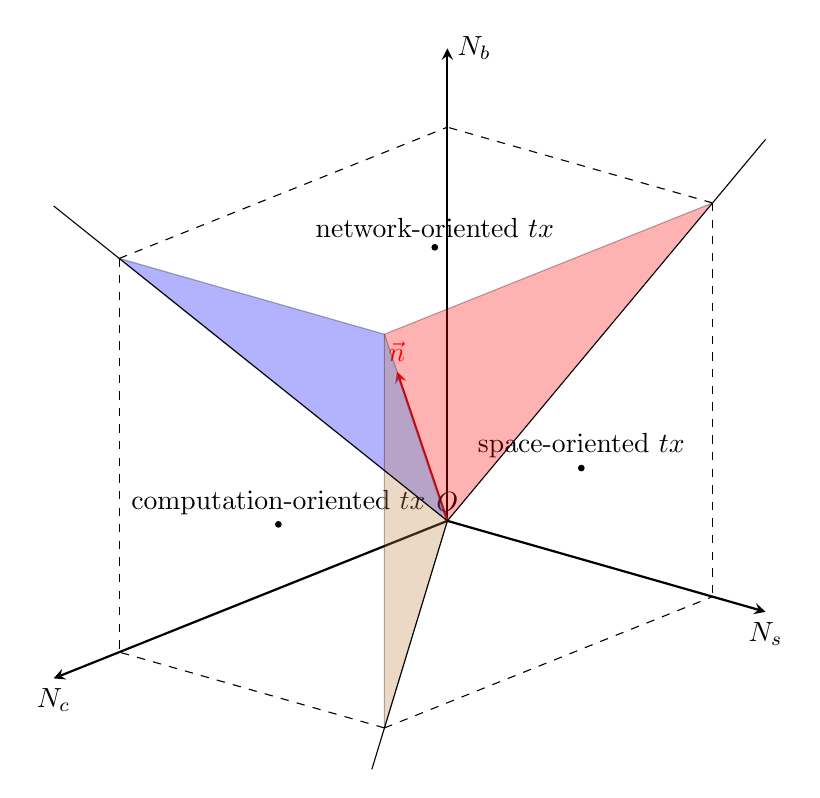
\begin{tikzpicture}[rotate around y=-30]
    \draw[thick,-stealth] (0,0,0)--(0,0,6) node [below] {$N_c$};
    \draw[thick,-stealth] (0,0,0)--(0,6,0) node [right] {$N_b$};
    \draw[thick,-stealth] (0,0,0)--(6,0,0) node [below] {$N_s$};
    \draw[thick,-stealth,red] (0,0,0)--(4,4,4) node [above] {$\vec{n}$};                                                                           

    \coordinate[label=$O$] (O) at (0,0,0);
    \coordinate[] (X) at (5,5,5);
    \coordinate[] (A) at (0,5,5);
    \coordinate[] (B) at (5,5,0);
    \coordinate[] (C) at (5,0,5);                                                                                                                  

    \draw plot [mark=*, mark size=1] coordinates{(5,2.3,2)} node[above]
    {space-oriented $tx$};
    \draw plot [mark=*, mark size=1] coordinates{(3,2.2,5)} node[above]
    {computation-oriented $tx$};
    \draw plot [mark=*, mark size=1] coordinates{(1,4,1)} node[above]
    {network-oriented $tx$};                                                                                                                       

    \draw[fill=blue,opacity=0.3] (X)--(A)--(O);
    \draw[fill=red,opacity=0.3] (B)--(X)--(O);
    \draw[fill=brown,opacity=0.3] (X)--(C)--(O);
    \draw[dashed] (A)--(0,0,5);
    \draw[dashed] (A)--(0,5,0);
    \draw[] (O)--(0,6,6);
    \draw[dashed] (B)--(5,0,0);
    \draw[dashed] (B)--(0,5,0);
    \draw[] (O)--(6,6,0);
    \draw[dashed] (C)--(5,0,0);
    \draw[dashed] (C)--(0,0,5);
    \draw[] (O)--(6,0,6);
\end{tikzpicture}
\end{document}
